\chapter{Assurance Cases and Selected Evidence for AortaGeomRecon}

\section{Assurance Case Development}

Assurance Case shows the statements and the evidences to ensure the goals are fulfilled. By using Astah GSN drawing software, we have a Tree view of our assurance case.

\section{Assurance Case for Software Specification Requirements}

The first goal of having a trusted software is a complete, consistant, unambiguous, cTODO Software Specification Requirements \citep{SRS} which shows the complete breakdown of the requirements with mathematical notation, data models and instance models.

As explains in the assurance case GR, the Software Specification Requirement having these characteristics by using a standard template. This template is provided by the domain expert Spencer Smith.

The chapters in SRS and some of the most important sections in the chapter are explained below:
\begin{itemize}
\item Reference Material

In this setion, a Table of Symbols and a Abbreviations and Acronyms table are used to explain every symbol and Abbreviations used in the SRS document. These tables ensures the consistancy and the unambiguous characteristics of the document. They are located at the very beginning of the document, so the reader will firstly look at these tables before reading the entire document.

\item Introduction

In the introduction section, we introduced the problems and the scope of the document to the user by explaining the purpose of document, abstracting the scope of requirements and defining the characterstics of intended reader. 

\item General System Description

The general system description includes a system context diagram which explains the relationship between the users, the inputs given by the user and the outputs of the AortaGeomRecon program. User responsibility and AortaGeomRecon responsibility are defined such that the user knows what to do to successfully generate the desired result. 

\item Specific System Description

In this section, we are presenting more details about the problem and the specific system to solve the problem. The first subsection Problem Description disucssed on the definition of Organ Segmentation, Coordinate Systems related to Human Organs visualization, Physical System Description which is not available, and Goal Statements which is extract the three-dimensional segmentation of the aorta.

In the next subsection, Solution Charateristics Specification, we started with Assumptions to simplify the problem and helps in developing the theoretical model by filling in the missing information for the physical systems. In the subsection Data Definitions, we defined Voxel, Image/Slice, and Volume with mathematical notation so that the developer can easily interpret. Next, in the subsection Instance Model, we showed the mathematical meaning of Region of Interest, and Segmentation, which are the two essential terms that the developer must know in order to develop the solution.


\begin{figure}[H]
    \centering
    \fbox{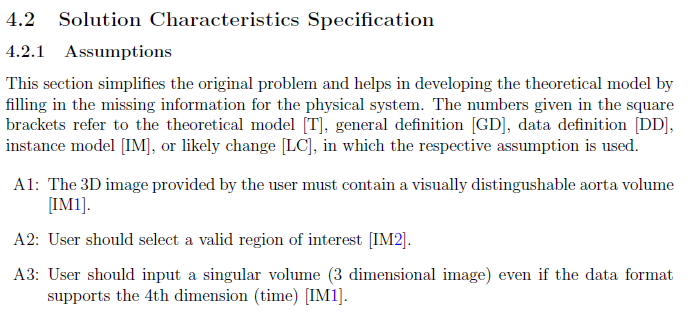
\includegraphics[width=0.8\textwidth]{figures/AC/SRS/Assumptions.png}}
    \caption[AortaGeomRecon SRS Assumptions]{AortaGeomRecon SRS Assumptions}
    \label{fig_agr_srs_a}
\end{figure}


\item Requirements

With all the information in the document, we can now present the Functional Requirements and the Non-Functional Requirements for the program AortaGeomRecon. The Functional Requirements are defined By using the terms we presented in Data Definitions, Instance Model, and based on the other Functional Requirements. The Non-Functional Requirements usually have a measurement such as execution time, the effort of manual works, etc.

\begin{figure}[H]
    \centering
    \fbox{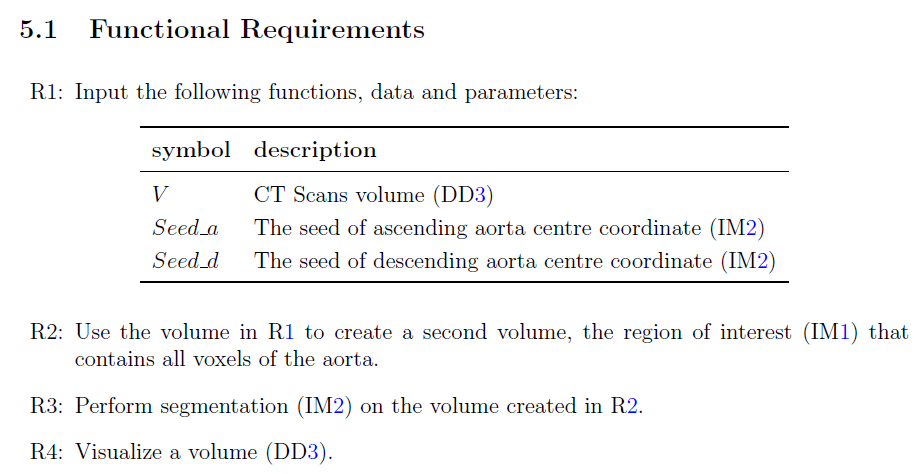
\includegraphics[width=0.7\textwidth]{figures/AC/SRS/Functional_Requirements.png}}
    \caption[AortaGeomRecon Functional Requirements]{AortaGeomRecon Functional Requirements}
    \label{fig_agr_fr}
\end{figure}

\begin{figure}[H]
    \centering
    \fbox{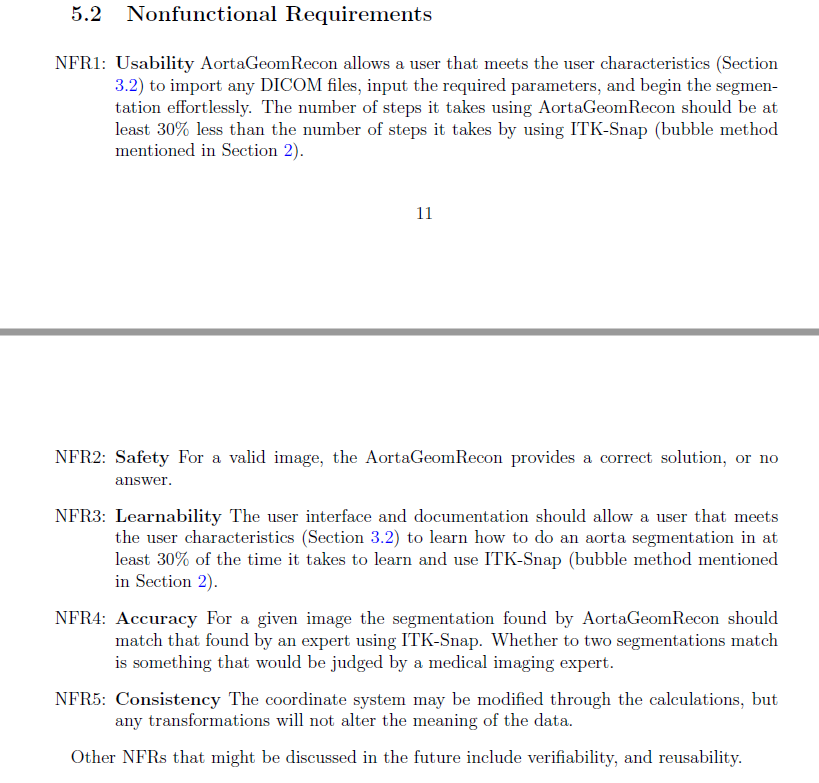
\includegraphics[width=0.7\textwidth]{figures/AC/SRS/NonFunctional_Requirements.png}}
    \caption[AortaGeomRecon Non- Functional Requirements]{AortaGeomRecon Non- Functional Requirements}
    \label{fig_agr_nfr}
\end{figure}

\item Likely Changes and Unlikely Changes

This section discussed the likely changes that the developer might expect a change in the future works, and the unlikely changes that is most certainly not going to change for a justified reason. The only likely change discussed in the AortaGeomRecon's SRS is regarding the segmentation method. For different segmentation method, the inputs varies, since the segmentation method is a likely change, the inputs variables are also likely changes. The only unlikely change is the method of retrieve a region of interest. Most methods takes a starting point and sizes in different dimensions to get the region of interest.

\item Traceability Matrix and Graphs

The traceability matrices is to provide easy references on what has to be additionally modified if a certain component is changed. Below shows the traceability matrices of different sections:
\begin{figure}[H]
    \centering
    \fbox{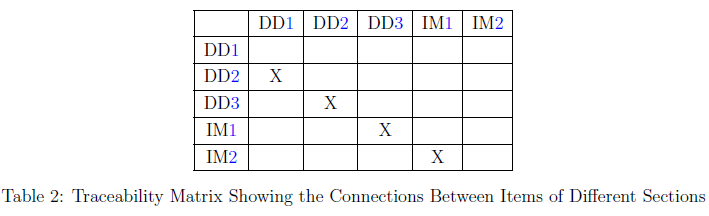
\includegraphics[width=0.7\textwidth]{figures/AC/SRS/tm_dd_im.png}}
    \caption[AortaGeomRecon Traceability Matrix between Data Definitions and Instance Model]{AortaGeomRecon Traceability Matrix between Data Definitions and Instance Model}
    \label{fig_agr_tm_dd_im}
\end{figure}

\begin{figure}[H]
    \centering
    \fbox{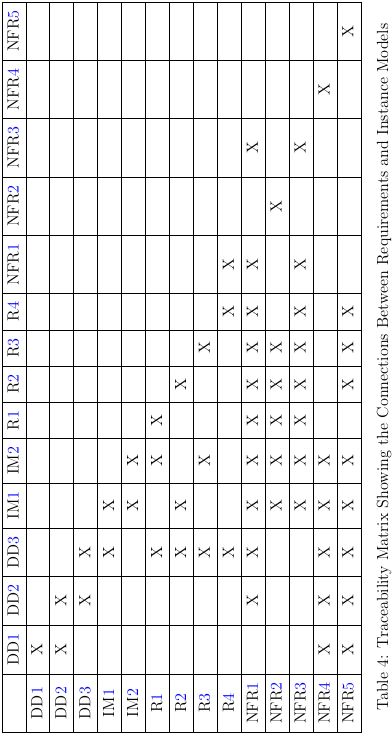
\includegraphics[width=0.7\textwidth]{figures/AC/SRS/tm_im_r.png}}
    \caption[[AortaGeomRecon Traceability Matrix between Requirements and Other sections]{AortaGeomRecon Traceability Matrix between Requirements and Other sections}
    \label{fig_agr_tm_im_r}
\end{figure}

\begin{figure}[H]
    \centering
    \fbox{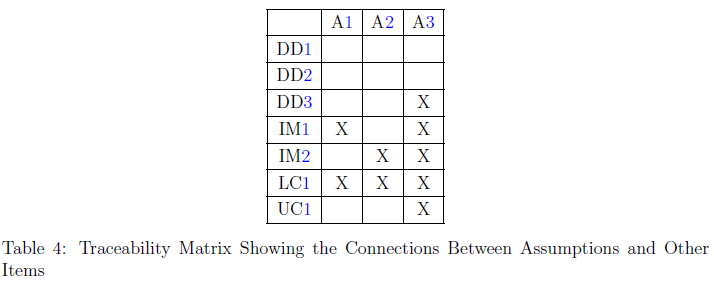
\includegraphics[width=0.7\textwidth]{figures/AC/SRS/tm_a.png}}
    \caption[AortaGeomRecon Traceability Matrix between Assumptions and Other sections]{AortaGeomRecon Traceability Matrix between Assumptions and Other sections}
    \label{fig_agr_tm_a}
\end{figure}


\end{itemize}

\section{Assurance Case for Implementation}
The goal of implementation asked the developer to fully comply the design and the implementation with the Software Requirements Specification document. Since we have showed with Assurance Case that our SRS is complete, consistant, and unambiguous, the design and the implementation that fully complying with requirements is correct.

\subsection{Design Document}
The purpose of the Design Document is to explain in details how the algorithm works, and why it worked. Similar to what section \ref{algo} wrote, the design document explains in plan text the workflow of the algorithm. Since before the domain expert can agree on the design and implementation, he/shee needs to understand the algorithm, we are building a Design Document that is easy to access. 

\subsubsection{Sphinx - Python Documentation Generator}
To implement this Design Document, I used Sphinx, a Python Documentation Generator that can build module's documentation with the comments in the source code. Moreover, using reStructuredText to write the Algorithm Overview, we can build html binary which can be publish on a webserver, which I was able to implement and accomplish. Another important section in Design Document is the Glossary. It has rich vocubulary explanation, images, and links to the outside source to let the reader understands as much as possible.

\subsection{Module Guide}
Module Guide is a document that support the modulization of the program. By doing the module decomposition, we have separate of concerns for each module. Sometimes, modules are tight to one or multiple requirements, we have built a Traceability Matrix between Modules and Requirements, Modules and Source code such that we trust all pieces of the source code are built for a reason, and they are built correctly.

% TODO: add TM images

Test Case
\begin{itemize}
\item GitHub Workflow
\item Continuous Integration tests
\begin{itemize}
\item build ``Ground Truth Data''
\item Steps
\item Coverage
\end{itemize}
\end{itemize}

\section{Algorithm Review}

The algorithm review was an idea started with Code Walkthrough. The difference is that Code Walkthrough aims to increase the confidence of the reviewer such that the reviewed implementation is doing what we have discussed. For an Algorithm Review, we have not discussed what the program should do; we are presenting the algorithm to the domain expert and aksing them if the design and implementation fullfill our requirements.

\subsection{Algorithm Review with Kailin Chu}
The first algorithm review was done with Kailin Chu, who is a biomedical engineer and started the semi-automacial aorta segmentation algorithm. Along with Smith Spencer, we were aiming to increase the domain expert's confidence in this code walkthrough. For various reaseon, this code walkthrough has not been successful, this implies that the domain expert has not gain confidence over the implementation. However, this meeting was helpful, because knowing that the algorithm might have flaw, I was able to iterate the algorithm and reaching a better result in a more efficient way.

\subsection{Algorithm Review with Dr. Dean Inglis}

The second algorithm review was done with Dr. Dean Inglish, who is a biomedical engineer and started the semi-automacial aorta segmentation algorithm. Along with Smith Spencer, we were aiming to increase the domain expert's confidence in this code walkthrough. For various reaseon, this code walkthrough has not been successful, this implies that the domain expert has not gain confidence over the implementation. However, this meeting was helpful, because knowing that the algorithm might have flaw, I was able to iterate the algorithm and reaching a better result in a more efficient way.
\subsubsection{}


\begin{itemize}
\item Python Spyder IDE - Data Visualization and Debugging tool
\item 
\item 
\end{itemize}


%\section{Referencing}
%These are some sample references to GAMYGDALA~\citep{popescu2014gamygdala} from 
%the \texttt{references.bib} file and state effects of 
%cognition~\citep{hudlicka2002time} from the \texttt{references\_another.bib} 
%file. These references are not in the same .bib file.
%
%\section{Figures}
%This is a single image figure (Figure~\ref{fig_singleenv}):
%
%\begin{figure}[ht]
%    \centering
%    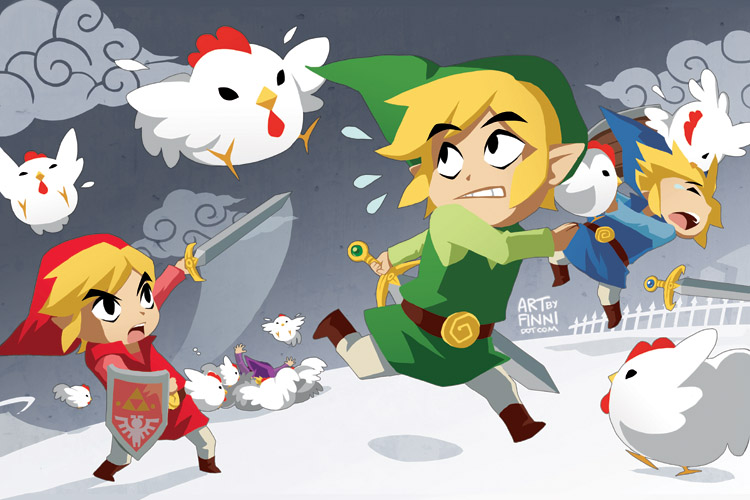
\includegraphics[width=0.6\textwidth]{figures/Sample/tumblr_static_eaceks0rfxsss8o4swscw40wo.jpg}
%    \caption[Single Figure Environment Listed Title]{This is a single figure 
%    environment}
%    \label{fig_singleenv}
%\end{figure}
%
%This is a multi-image figure with a top (Figure~\ref{fig_multienv_1}) and bottom (Figure~\ref{fig_multienv_2}) aligned subfigures:
%
%\begin{figure}[ht]
%	\centering
%	\begin{subfigure}[t]{\textwidth}
%		\centering
%		
%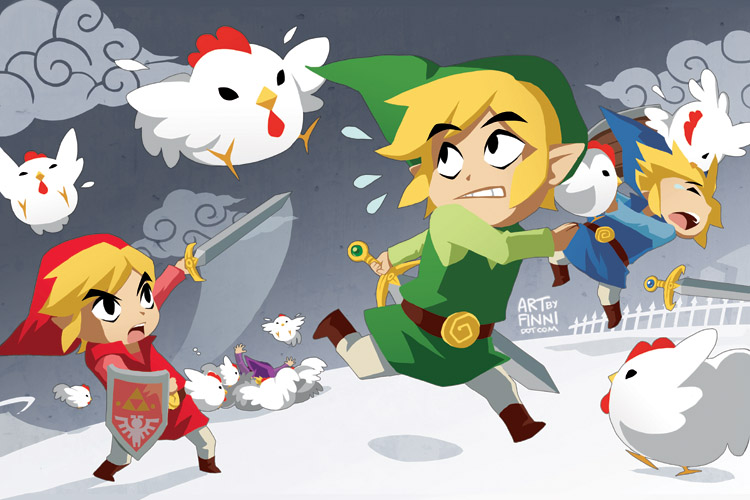
\includegraphics[width=0.7\textwidth]{figures/Sample/tumblr_static_eaceks0rfxsss8o4swscw40wo.jpg}
%		\caption{Figure 1}
%		\label{fig_multienv_1}
%	\end{subfigure}
%	~
%	\begin{subfigure}[t]{\textwidth}
%		\centering
%		
%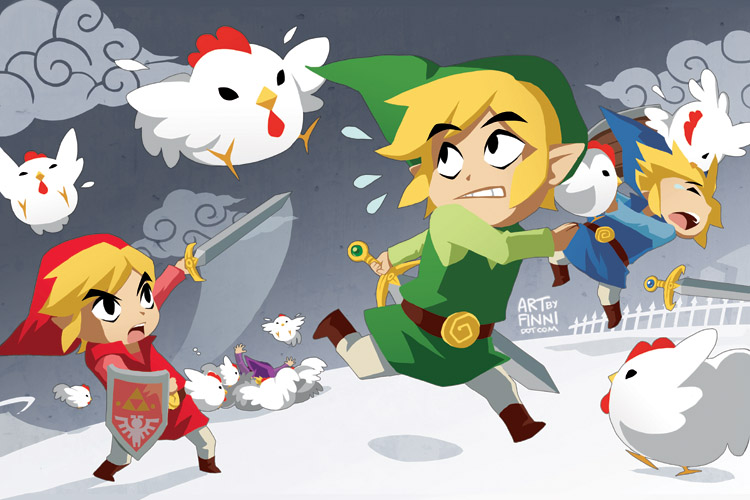
\includegraphics[width=0.7\textwidth]{figures/Sample/tumblr_static_eaceks0rfxsss8o4swscw40wo.jpg}
%		\caption{Figure 2}
%		\label{fig_multienv_2}
%	\end{subfigure}
%	
%	\caption{A Multi-Figure Environment}
%	\label{fig_multienv}
%\end{figure}
%
%\section{Tables}
%
%Here is a sample table (Table~\ref{tab_sample}):
%
%	\begin{table}[ht]
%	\centering
%	\begin{tabular}{ m{0.2\textwidth} m {0.1\textwidth} m{0.15\textwidth} }
%		\toprule
%		A & $\longleftrightarrow$ & B \\
%		C & $\longleftrightarrow$ & D \\
%		\bottomrule	
%	\end{tabular}	
%	\caption{A sample table}	
%	\label{tab_sample}
%\end{table}
%
%\subsection{Long Tables}
%A sample long table is shown in Appendix~\ref{appendix_b}.
%
%\section{Equations}
%
%Here is a sample equation (Equation~\ref{eq_lineslope}):
%
%\begin{equation} \label{eq_lineslope}
%	y = mx + b
%\end{equation}